\documentclass[a4paper,oneside,openright,11pt]{book}

\usepackage[T1]{fontenc}

%%%%%%%% Schriftart Latin Modern verwenden:
\usepackage{lmodern}
\usepackage[utf8]{inputenc} % ggf. Editor auf utf8 stellen!!
\usepackage[ngerman]{babel}
\usepackage{ngerman} % unter anderem für bessere Silbentrennung
\usepackage{listings}
\usepackage{amssymb}
\usepackage{amsmath}
\usepackage{graphicx}
\usepackage{url}
\def\UrlBreaks{\do\/\do-} % Zeilenumbrüche in URLs bei Bindestrich oder Schrägstrich
\usepackage{hyperref}
\usepackage{xspace}
\usepackage{csquotes}
\usepackage{fancyhdr}
\usepackage{titlesec}
\usepackage{todonotes}
\usepackage{multirow}
\usepackage{bigstrut}
\usepackage{subcaption}



%avoid overfull hbox problem
\setlength{\emergencystretch}{3em}

%avoid underfull hbox problem in bibliography
\usepackage{etoolbox}
% Variant A
\apptocmd{\sloppy}{\hbadness 2000\relax}{}{}
% Variant B
% \apptocmd{\thebibliography}{\raggedright}{}{}
\hyphenpenalty=5000
\tolerance=1000

% standard scaling factor for graphics, to support homogenous looks.
\newcommand{\stdScaleFactor}{0.45}

% Titelseite und Erklaerung
\usepackage{sethesis}

% Angaben Titelseite
\unilogo{
\includegraphics[scale=0.75]{FHDW-Logo.eps}}
% Angaben zur Arbeit
\author{Yashar Busch\\Oliver Gröne\\Amelie Meyer\\Daniel Pasternak} % Hier Namen eintragen
\title{Einführungsaufgaben 10 \& 11} % Hier Titel
\version{07-08-2026}
\ort{Hannover}

\datum{\today} % Datum der Abgabe hier einsetzen

\begin{document}

\frontmatter

\maketitle

\clearpage
%%%%%% Sperrvermerk einkommentieren, falls nötig.
%\input{restriction-notice}

\clearpage
% \chapter*{Changemanagment}

\begin{table}[h!]
\centering
\renewcommand{\arraystretch}{1.3}
\begin{tabular}{|p{7cm}|p{3cm}|p{3cm}|}
\hline
\textbf{Änderung} & \textbf{Autor} & \textbf{Datum} \\
\hline
Initiale Erstellung des Dokuments & E. Karakaya & 24.01.2026 \\
\hline
 &  &  \\
\hline
 &  &  \\
\hline
\end{tabular}
\end{table}

\tableofcontents
\mainmatter

\chapter{Aufgabe 10 - Konzept des Schedulers}
Im Konzept des Schedulers gehen wir auf die Tasks, Scheduling-Periode, die Stacks und die Spezialfunktionsregister (SFR) ein.

\section{Scheduling-Periode}
\label{subsec:schedulingPeriode}
Die Scheduling-Periode beträgt 2,5 ms.
Somit ist die Echtzeitanforderung von 10 ms für den Reaktions-Task gegeben, da jeder Task maximal 2,5 ms läuft, was bei 4 Tasks summiert 10 ms sind.

Wir verwenden Timer 0 im Modus 1 (16-Bit Timer).
Timer 0 muss bei jedem Aufruf eines Tasks neu gesetzt werden, da in dem Modus der Timer nicht automatisch Nachladen kann und wir ggf. auch vor einem Überlauf in einem alten Task in einen neuen Task wechseln.
Timer 0 wird auf den Wert \verb|0xF36C| bzw. \verb|63.036| gesetzt.

\subsection{Einflussparameter}
Die Aufgabenstellung verlangte über verschiedene Einflussparameter auf die Scheduling-Periode zu diskutieren.
\begin{description}
    \item[Hitze]
    Durch Hitze kann es zu einer Verlangsamung des Systems bzw. des Timers kommen.
    Dies kann zu einer Verlängerung der Scheduling-Periode führen.
    \item[Interrupts]
    Sollten im Zuge einer Umstellung der Tasks andere Interrupts eingeschaltet werden, so kann es dazu kommen, dass der Timer 0 Interrupt erst verspätet abgearbeitet wird.
    Dies kann zu einer Verlängerung der Scheduling-Periode führen.
\end{description}

\section{Tasks}
Jeder Task (einschließlich des Schedulers) hat eine eigene Registerbank zugewiesen (siehe bei den Taskbeschreibungen die Eckdaten).
In der Registerbank des Schedulers bekommt jeder Task außerdem ein eigenes Register, in welchem wir die Stackpointer (SP) der jeweiligen Tasks speichern und auch auf diesen laden.
Im Folgenden schauen wir uns die Tasks im einzelnen genauer an.

\subsection{Scheduler}
Der Scheduler kümmert sich um den Wechsel der Tasks bzw. des Kontexts und besitzt dazu seinen eigenen Kontext.
Er sitzt in der Interrupt-Routine von Timer 0, unserem Scheduling-Periode-Timer.

Beim Aufruf des Schedulers wird automatisch, da es eine Interrupt Routine ist, der Programcounter (PC) auf den Stack des alten Tasks geschrieben.
Innerhalb des Schedulers werden dann die SFR ebenfalls auf den Stack geschrieben (Reihenfolge: Akkumulator, B-Register, Programmstatuswort (PSW)-Register, Datapointer (DPTR)-Lowbyte (DPL) und DPTR-Highbyte (DPH)), die Registerbank wird zu der des Schedulers gewechselt und der SP des alten Tasks wird in das ihm zugewiesene Register gespeichert.

Im Folgenden wählt der Scheduler den nächsten Task, wechselt den Stack zum neuen Task, liest die SFR vom Stack und beendet die Interrupt-Routine, sodass der PC einfach wieder vom Stack gelesen wird und der Task da weitermachen kann, wo er aufgehört hat.

Zusammengefasst noch einmal der Ablauf des Schedulers:
\begin{enumerate}
    \item Pushen der SFR auf den Stack des alten Tasks
    \item Wechseln der Registerbank zu der dem Scheduler zugehörigen
    \item Laden des Stacks des Schedulers
    \item Laden der SFR aus dem Scheduler Stack
    \item Nächsten Task auswählen
    \item Pushen der SFR auf den Scheduler Stack
    \item Laden des Stacks des neuen Tasks
\end{enumerate}
Eckdaten des Schedulers:
\begin{description}
    \item[Stackpointer (Init):] \verb|0x80|
    \item[Registerbank:] \verb|0x00|
    \item[Register für SP:] R4 bzw. \verb|0x04|
\end{description}

\subsection{Uhr-Task}
Den Uhr-Task haben wir bereits in einer vorherigen Aufgabe erstellt, weshalb eine genau Erklärung der Funktionsweise hier ausbleibt und nur die Änderungen erklärt werden.

In der Vorlesung wurde sich darauf geeinigt, dass der Uhr-Task statt wie vorher mit dem Timer 0 und per Interrupt maximal alle 250 µs schaltet, nun mit dem Timer 2 und alle 50 ms schalten soll.
Durch die Aufgabenstellung war außerdem vorausgesetzt, dass der Scheduler \glqq als einziger Task mit Hilfe eines Interrupts gesteuert wird.\grqq

Durch diese Voraussetzungen wurde der Uhr-Task so abgeändert, dass wir ...
\begin{itemize}
    \item ... keinen Interrupt verwenden, sondern bei jedem Aufruf des Uhr-Tasks das Interrupt-Bit abfragen,
    \item bei gesetztem Interrupt-Bit die Uhr hochzählen und das Interrupt-Bit zurücksetzen,
    \item bei nicht gesetztem Interrupt-Bit wird direkt an den Scheduler abgegeben und
    \item statt der vorherig maximal 250 µs jetzt 50 ms hochzählen.
\end{itemize}
Eckdaten des Uhr-Tasks:
\begin{description}
    \item[Stackpointer (Init):] \verb|0xA0|
    \item[Registerbank:] \verb|0x01| 
    \item[Register für SP:] R5 bzw. \verb|0x05| 
\end{description}

\subsection{Reaktions-Task}
Der Reaktions-Task \glqq berechnet, ob der binäre 8-bit Wert an einem festzulegenden Port größer als 200 oder kleiner als 100 ist. Diese Information wird durch zwei Bits eines anderen festzulegenen Ports mindestens alle 10 ms aktualisiert.\grqq\ 
Für die Ports haben wir uns als Eingabe (8-Bit) für Port 1 entschieden.
Als Ausgabe benutzen wir P3.2 (XH) und P3.3 (XL).
Die Echtzeitanforderungen erfüllen wir wie in \autoref{subsec:schedulingPeriode} erklärt.
Außerdem haben wir uns dazu entschieden, bei Aufruf des Reaktions-Task den Wert des vorherigen Aufrufs gegen den Wert des aktuellen Aufruf zu vergleichen und bei Gleichheit direkt an den Scheduler abzugeben, um so CPU Zeit zu sparen.
Dafür wird der anliegende Wert in R0 zwischengespeichert.

Eckdaten des Reaktions-Task:
\begin{description}
    \item[Stackpointer (Init):] \verb|0xC0|
    \item[Registerbank:] \verb|0x10| 
    \item[Register für SP:] R6 bzw. \verb|0x06| 
\end{description}

\subsection{Berechnungs-Task}
Im Berechnungs-Task \glqq werden alle Speicherzellen des externen RAMs entsprechend der Größe sortiert.\grqq\ 
Der Einfachheit halber haben wir uns hier für einen Bubble-Sort entschieden.
Wir vergleichen also immer die aktuelle Zelle mit der nächsten Zelle im externen RAM und tauschen, sofern die aktuelle Zelle größer ist.
Eckdaten des Berechnungs-Tasks:
\begin{description}
    \item[Stackpointer (Init):] \verb|0xE0|
    \item[Registerbank:] \verb|0x11| 
    \item[Register für SP:] R7 bzw. \verb|0x07| 
\end{description}

\section{Initialisierung}
In der Initialisierung müssen verschiedene Werte gesetzt werden.
Am Ende muss das Interrupt-Bit für Timer 0 gesetzt werden, um den Scheduler aufzurufen.

Die Initialisierung der Stacks ist dabei besonders.
Hier ist auf eine gewisse Struktur zu achten, um später einen reibungslosen Ablauf im Scheduler zu gewährleisten.
Die Struktur sieht wie folgt aus:
\begin{enumerate}
    \item PC-Lowbyte
    \item PC-Highbyte
    \item Akkumulator
    \item B-Register
    \item PSW-Register
    \item DPL-Register
    \item DPH-Register
\end{enumerate}
Die PC-Werte werden dynamisch durch die Label der Unterprogramme gesetzt.
Das PSW-Register wird so initialisiert, dass es direkt auf die dem Task zugewiesene Registerbank zeigt.
Alle anderen Register werden mit \verb|0x00| initialisiert.

Der Ablauf ist im Folgenden beschrieben:
\subsection{Stackpointer}
Zuallererst wird der SP auf den Stack des Schedulers gesetzt.
Unser SP für den Scheduler beginnt bei \verb|0x80| und wird daher auf \verb|0x7F| gesetzt.

\subsection{Timer 0}
Timer 0 muss auf den Modus 1 (16-Bit) geschaltet werden.
Er wird mit \verb|0xF36C| geladen und gestartet.

\subsection{Timer 2}
Timer 2 wird im Nachlademodus betrieben.
Es müssen Timer 2 und die Nachladeregister des Timer 2 mit \verb|0x3CB0| geladen werden.
Der Timer wird gestartet.

\subsection{Interrupts}
Es wird der Interrupt für Timer 0 eingeschaltet.
Es wird die globale Interruptfreigabe gesetzt.

\subsection{Scheduler}
Es wird in A \verb|0x04| geschrieben.

\subsection{Uhr-Task}
Der SP des Uhr-Task beginnt bei \verb|0xA0|, wir setzen also SP als Nächstes auf \verb|0x9F|.
Es werden die folgenden Werte auf den Stack geschrieben:
\begin{itemize}
    \item Lowbyte Programmlabel
    \item Highbyte Programmlabel
    \item Akkumulator (\verb|0x00|)
    \item B-Register (\verb|0x00|)
    \item PSW-Register (\verb|0x08|)
    \item DPL-Register (\verb|0x00|)
    \item DPH-Register (\verb|0x00|)
\end{itemize}
Der SP (nun \verb|0xA6|) wird im zugehörigem Register (R5) gespeichert.

\subsection{Reaktions-Task}
Der SP des Reaktions-Task beginnt bei \verb|0xC0|, wir setzen also SP als Nächstes auf \verb|0xBF|.
Es werden die folgenden Werte auf den Stack geschrieben:
\begin{itemize}
    \item Lowbyte Programmlabel
    \item Highbyte Programmlabel
    \item Akkumulator (\verb|0x00|)
    \item B-Register (\verb|0x00|)
    \item PSW-Register (\verb|0x10|)
    \item DPL-Register (\verb|0x00|)
    \item DPH-Register (\verb|0x00|)
\end{itemize}
Der SP (nun \verb|0xC6|) wird im zugehörigem Register (R6) gespeichert.

\subsection{Berechnungs-Task}
Der SP des Berechnungs-Task beginnt bei \verb|0xE0|, wir setzen also SP als Nächstes auf \verb|0xDF|.
Es werden die folgenden Werte auf den Stack geschrieben:
\begin{itemize}
    \item Lowbyte Programmlabel
    \item Highbyte Programmlabel
    \item Akkumulator (\verb|0x00|)
    \item B-Register (\verb|0x00|)
    \item PSW-Register (\verb|0x18|)
    \item DPL-Register (\verb|0x00|)
    \item DPH-Register (\verb|0x00|)
\end{itemize}
Der SP (nun \verb|0xE6|) wird im zugehörigem Register (R7) gespeichert.

\chapter{Aufgabe 11 - Monitoring}
\section{Unterschiedliche Ansätze des Monitorings}
\begin{table}[ht]
    \centering
    \begin{tabular}{ p{3cm} | p{4cm} | p{5cm} }
         \textbf{Monitoring Ansatz}&
         \textbf{Vorteile} &
         \textbf{Nachteile} \\
         
         \hline
         \hline
         \multirow[c]{4}{=}{\textbf{Software-Monitoring}} &
         \begin{itemize}
             \item Einfach zu implementieren
             \item Keine zusätzliche Hardware erforderlich
         \end{itemize} &
         \begin{itemize}
             \item Zugriff auf Kernel-Ebene benötigt
             \item Höherer Zeitbedarf und Ressourcennutzung
             \item Möglicherweise veraltete Daten
             \item (mögliche) Beeinträchtigung des Echtzeit-Verhaltens
         \end{itemize} \\

         \hline
         \multirow[c]{4}{=}{\textbf{Hybrid-Monitoring}} &
         \begin{itemize}
             \item Geringerer CPU-Overhead
             \item Gute Balance zwischen Kosten/Genauigkeit
         \end{itemize} &
         \begin{itemize}
             \item Zusätzliche Hardware benötigt
             \item Anpassungen im Quellcode notwendig
         \end{itemize} \\

         \hline
         \multirow[c]{4}{=}{\textbf{Hardware-Monitoring}} &
         \begin{itemize}
             \item Unabhängig, da keine Systemressourcen benötigt werden
         \end{itemize} &
         \begin{itemize}
             \item Zusätzliche Hardware benötigt
             \item Spezielles Werkzeug notwendig aufgrund der Größe
         \end{itemize}
    \end{tabular}
\end{table}
\newpage
Das Software-Monitoring ist zwar einfach zu implementieren, jedoch verliert es in Sachen Performance und Genauigkeit, da die Daten über mehrere Ebenen durchgereicht werden und zudem eine Umwandlung von analog in digital geschieht, wodurch es zu Ungenauigkeiten kommt.

Beim Hybrid-Monitoring ist die Balance zwischen Leistung/Effizienz.
Die eigentliche Messung geschieht über Hardware-Sensorik, jedoch muss der Quellcode angepasst werden, um diese Daten auslesen zu können.
Daher bietet sich dies als Kompromiss an, falls Leistung \glqq über\grqq ist.

Das Hardware-Monitoring ist am schnellsten, da keine zusätzlichen Ebenen benötigt werden, um die Daten auszulesen.
Zudem ist die Genauigkeit ebenfalls höher, da die analogen Signale nicht in digitale umgewandelt werden müssen.

\section{Konzept eines Software-Monitoring für 8051}
\paragraph{eine Stunde}
Unsere Idee ist im internen RAM je Task vier Byte zu reservieren.
Timer 1 zählt dann zur Laufzeit des jeweiligen Tasks mit.
Wenn der Task gewechselt wird, wird die gelaufene Zeit aufaddiert und die Zellen gewechselt.
Damit können wir einen unsigned integer mit 32-Bit speichern, dessen Wert in ms ca. einer Stunde und zwölf Minuten entspricht.

\paragraph{sechs Monate}
Das Vorgehen entspricht dem vorherigen.
Dafür benötigen wir ca. 5,5 Byte.
Diese runden wir auf sechs Byte auf.
Mit dieser Anzahl wären wir sogar in der Lage 108 Monate zu speichern.

\section{Laufzeitsimulation}
\begin{figure}[ht]
    \centering
    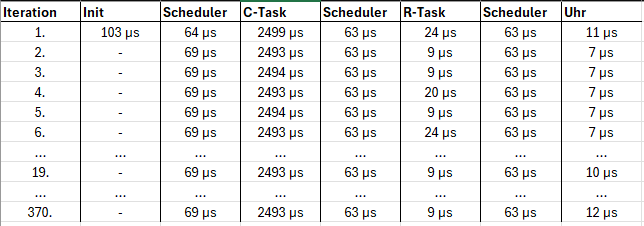
\includegraphics[width=\linewidth]{ressources/aufgabe11/Beispieliterationen mit Extrapolation.png}
    \caption{Laufzeiten der Tasks mit Extrapolation}
    \label{fig:iterationMitExtrapolation}
\end{figure}

\begin{figure}[ht]
    \centering
    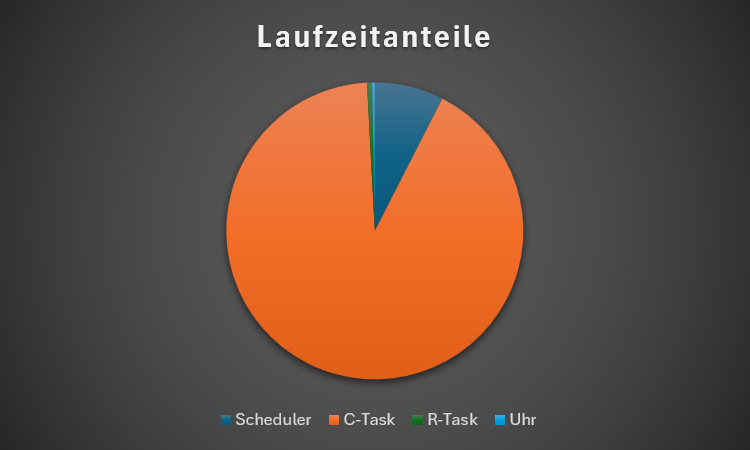
\includegraphics[width=0.9\linewidth]{ressources/aufgabe11/Laufzeitanteile.png} 
    \caption{Laufzeitanteile}
\end{figure}

\begin{figure}
    \centering
    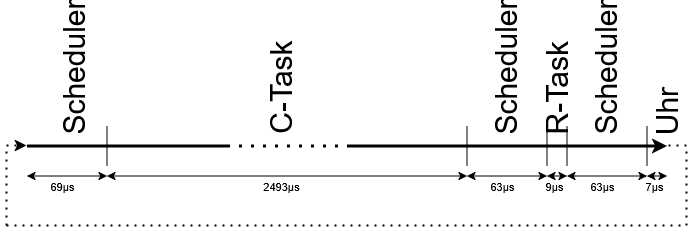
\includegraphics[width=\linewidth]{ressources/aufgabe11/Zeitverlauf_Beispiel.png}
    \caption{Zeitverlauf wiederkehrend}
\end{figure}



\appendix

\input{contents/anhang}

%\bibliographystyle{alpha}
\bibliographystyle{halpha-abbrv} % Support curstom abbreviation labels, see https://www.math.cmu.edu/~gautam/sj/blog/20171114-bibtex-doi.html
\bibliography{meinearbeit}

\backmatter


\end{document}